\documentclass[conference]{IEEEtran}
\IEEEoverridecommandlockouts

\usepackage{cite}
\usepackage{amsmath,amssymb,amsfonts}
\usepackage{graphicx}
\usepackage{booktabs}
\usepackage{multirow}
\usepackage{xcolor}
\usepackage{tikz}
\usetikzlibrary{positioning,arrows.meta,fit,backgrounds}
\usepackage[hidelinks]{hyperref}

% Auto-generated by paper_analysis.py -- do not edit by hand
\newcommand{\nRaw}{3,507}
\newcommand{\nBuy}{1,399}
\newcommand{\nWS}{1,308}
\newcommand{\nTick}{393}
\newcommand{\nDays}{116}
\newcommand{\nUniv}{499}
\newcommand{\dFirst}{2026-01-09}
\newcommand{\dLast}{2026-09-10}
\newcommand{\dEvalEnd}{2026-09-24}
\newcommand{\medRSI}{43.1}
\newcommand{\meanConf}{0.82}
\newcommand{\sigPerDay}{12.1}
\newcommand{\spyTotal}{+11.4}
\newcommand{\mBuyRawten}{+1.71}
\newcommand{\mBuyRawtenCI}{[+0.18, +3.46]}
\newcommand{\mBuyRawtenP}{0.020}
\newcommand{\mBuyExten}{-0.10}
\newcommand{\mBuyExtenCI}{[-1.06, +0.97]}
\newcommand{\mBuyExtenP}{0.838}
\newcommand{\mBuyCarten}{-0.04}
\newcommand{\mBuyCartenCI}{[-1.10, +1.04]}
\newcommand{\mBuyCartenP}{0.942}
\newcommand{\mMatchCarten}{+0.09}
\newcommand{\mMatchCartenCI}{[-1.05, +1.23]}
\newcommand{\mMatchCartenP}{0.840}
\newcommand{\mRandCarten}{-0.13}
\newcommand{\mRandCartenCI}{[-1.06, +0.76]}
\newcommand{\mRandCartenP}{0.772}
\newcommand{\mWsCarten}{+0.31}
\newcommand{\mWsCartenCI}{[-0.60, +1.15]}
\newcommand{\mWsCartenP}{0.482}
\newcommand{\mBuyMinusMatch}{-0.13}
\newcommand{\mBuyMinusMatchCI}{[-1.21, +0.93]}
\newcommand{\mBuyMinusMatchP}{0.803}
\newcommand{\mBuyMinusRand}{+0.09}
\newcommand{\mBuyMinusRandCI}{[-1.05, +1.22]}
\newcommand{\mBuyMinusRandP}{0.853}
\newcommand{\mMatchMinusRand}{+0.23}
\newcommand{\mMatchMinusRandCI}{[-0.21, +0.78]}
\newcommand{\mMatchMinusRandP}{0.417}
\newcommand{\mBuyCarfive}{-0.16}
\newcommand{\mBuyCarfiveCI}{[-0.99, +0.66]}
\newcommand{\mBuyCarfiveP}{0.729}
\newcommand{\mBuyHitten}{53.5}
\newcommand{\mBuyHittenCI}{[+46.90, +59.85]}
\newcommand{\mBuyHittenP}{$<$0.001}
\newcommand{\mMatchHitten}{62.9}
\newcommand{\mMatchHittenCI}{[+53.80, +72.36]}
\newcommand{\mMatchHittenP}{$<$0.001}
\newcommand{\holdNet}{+1.61}
\newcommand{\holdNetCI}{[+0.09, +3.36]}
\newcommand{\depNet}{-0.06}
\newcommand{\depNetCI}{[-0.31, +0.17]}
\newcommand{\depGap}{-1.67}
\newcommand{\depGapCI}{[-3.23, -0.27]}
\newcommand{\depGapP}{0.008}
\newcommand{\depStopRate}{65.5}
\newcommand{\depTgtRate}{32.9}
\newcommand{\depWin}{33.9}
\newcommand{\holdWin}{53.2}
\newcommand{\medStopPct}{1.87}
\newcommand{\medStopATR}{0.49}
\newcommand{\gridBest}{+1.61}
\newcommand{\gridWorst}{+0.12}
\newcommand{\ece}{0.366}
\newcommand{\brier}{0.386}
\newcommand{\brierBase}{0.247}
\newcommand{\calConf}{0.82}
\newcommand{\calWin}{44.9}
\newcommand{\rhoConf}{+0.008}
\newcommand{\rhoConfCI}{[-0.045, +0.064]}
\newcommand{\pLlmTot}{+17.4}
\newcommand{\pLlmVol}{14.0}
\newcommand{\pLlmSh}{1.70}
\newcommand{\pLlmMdd}{-7.7}
\newcommand{\pLlmAlpha}{+15.2}
\newcommand{\pLlmAlphaT}{0.94}
\newcommand{\pLlmBeta}{0.53}
\newcommand{\pMatchTot}{+9.4}
\newcommand{\pMatchVol}{13.8}
\newcommand{\pMatchSh}{1.00}
\newcommand{\pMatchMdd}{-7.8}
\newcommand{\pMatchAlpha}{+3.1}
\newcommand{\pMatchAlphaT}{0.26}
\newcommand{\pMatchBeta}{0.66}
\newcommand{\pRuleTot}{+8.8}
\newcommand{\pRuleVol}{19.8}
\newcommand{\pRuleSh}{0.71}
\newcommand{\pRuleMdd}{-13.5}
\newcommand{\pRuleAlpha}{+1.9}
\newcommand{\pRuleAlphaT}{0.09}
\newcommand{\pRuleBeta}{0.74}
\newcommand{\pSpyTot}{+11.4}
\newcommand{\pSpyVol}{13.4}
\newcommand{\pSpySh}{1.21}
\newcommand{\pSpyMdd}{-8.9}
\newcommand{\pSpyAlpha}{--}
\newcommand{\pSpyAlphaT}{--}
\newcommand{\pSpyBeta}{1.00}
\newcommand{\pLSTot}{+6.7}
\newcommand{\pLSVol}{12.3}
\newcommand{\pLSSh}{0.82}
\newcommand{\pLSMdd}{-7.1}
\newcommand{\pLSAlpha}{+10.0}
\newcommand{\pLSAlphaT}{0.68}
\newcommand{\pLSBeta}{--}
\newcommand{\rHone}{-0.07}
\newcommand{\rHoneCI}{[-0.29, +0.14]}
\newcommand{\rHthree}{-0.24}
\newcommand{\rHthreeCI}{[-0.91, +0.30]}
\newcommand{\rHfive}{-0.33}
\newcommand{\rHfiveCI}{[-1.40, +0.53]}
\newcommand{\rHonezero}{-0.13}
\newcommand{\rHonezeroCI}{[-1.19, +0.94]}
\newcommand{\rNextOpenEx}{-0.23}
\newcommand{\rNextOpenExCI}{[-1.29, +0.93]}
\newcommand{\rExclTopDecileRsi}{-0.16}
\newcommand{\rExclTopDecileRsiCI}{[-1.16, +0.89]}
\newcommand{\gridHalfNoTgt}{+0.32}
\newcommand{\regimeRows}{%
VIX$<$16 & 142 & -0.17 & -0.79 & [-1.46, -0.25] & 0.006 \\
16-20 & 925 & -0.34 & -0.58 & [-1.74, +0.51] & 0.308 \\
VIX$>$20 & 332 & +0.86 & +1.41 & [-1.23, +2.68] & 0.243 \\
SPY$>$SMA50 & 1087 & -0.31 & -0.62 & [-1.58, +0.36] & 0.212 \\
SPY$<$SMA50 & 312 & +0.90 & +1.56 & [-0.45, +2.82] & 0.098 \\
}
\newcommand{\calibRows}{%
$[0.0, 0.7)$ & 48 & 0.59 & 43.8 & 25.0 & +2.07 \\
$[0.7, 0.8)$ & 330 & 0.75 & 42.7 & 31.2 & -0.23 \\
$[0.8, 0.85)$ & 671 & 0.82 & 45.5 & 34.0 & -0.32 \\
$[0.85, 0.9)$ & 332 & 0.90 & 46.1 & 32.5 & +0.10 \\
$[0.9, 1.0]$ & 18 & 0.96 & 44.4 & 50.0 & -1.36 \\
}

% Auto-generated by paper_intraday.py -- do not edit by hand
\newcommand{\iN}{1,414}
\newcommand{\iDays}{119}
\newcommand{\iStop}{10.9}
\newcommand{\iTgt}{0.6}
\newcommand{\iHit}{50.6}
\newcommand{\iMatchHit}{48.3}
\newcommand{\iDepWin}{43.4}
\newcommand{\iRaw}{-0.06}
\newcommand{\iRawCI}{[-0.18, +0.06]}
\newcommand{\iRawP}{0.369}
\newcommand{\iEx}{-0.03}
\newcommand{\iExCI}{[-0.13, +0.06]}
\newcommand{\iExP}{0.478}
\newcommand{\iMatchEx}{+0.01}
\newcommand{\iMatchExCI}{[-0.04, +0.06]}
\newcommand{\iMatchExP}{0.729}
\newcommand{\iRandEx}{-0.04}
\newcommand{\iRandExCI}{[-0.07, +0.00]}
\newcommand{\iRandExP}{0.088}
\newcommand{\iAlpha}{-0.04}
\newcommand{\iAlphaCI}{[-0.12, +0.04]}
\newcommand{\iAlphaP}{0.294}
\newcommand{\iAlphaRand}{+0.00}
\newcommand{\iAlphaRandCI}{[-0.09, +0.10]}
\newcommand{\iAlphaRandP}{0.951}
\newcommand{\iHoldNet}{-0.16}
\newcommand{\iHoldNetCI}{[-0.28, -0.04]}
\newcommand{\iHoldNetP}{0.009}
\newcommand{\iDep}{-0.16}
\newcommand{\iDepCI}{[-0.27, -0.05]}
\newcommand{\iDepP}{0.004}
\newcommand{\iDepGap}{-0.00}
\newcommand{\iDepGapCI}{[-0.04, +0.04]}
\newcommand{\iDepGapP}{0.947}

% Auto-generated by paper_ops.py -- do not edit by hand
\newcommand{\opDecisions}{67,810}
\newcommand{\opReal}{19,467}
\newcommand{\opFallback}{48,343}
\newcommand{\opFallbackPct}{71.3}
\newcommand{\opRealPct}{28.7}
\newcommand{\opQuota}{48,340}
\newcommand{\opQuotaDays}{28}
\newcommand{\opActiveDays}{169}
\newcommand{\opQuotaFirst}{2026-02-06}
\newcommand{\opQuotaLast}{2026-05-18}
\newcommand{\opScans}{842}
\newcommand{\opLatMed}{9.4}
\newcommand{\opLatPtf}{19.3}
\newcommand{\opHttpOk}{36,864}
\newcommand{\opHttpLimited}{286,876}
\newcommand{\opJsonErr}{2}
\newcommand{\opScanMedMin}{1.6}
\newcommand{\opSelMed}{38}
\newcommand{\opBuyShare}{30.2}
\newcommand{\mdeSeIntra}{0.040}
\newcommand{\mdeIntra}{0.112}
\newcommand{\mdeUpperIntra}{+0.035}
\newcommand{\mdeSeOne}{0.110}
\newcommand{\mdeOne}{0.31}
\newcommand{\mdeUpperOne}{+0.14}
\newcommand{\mdeSeThree}{0.305}
\newcommand{\mdeThree}{0.85}
\newcommand{\mdeUpperThree}{+0.30}
\newcommand{\mdeSeFive}{0.491}
\newcommand{\mdeFive}{1.38}
\newcommand{\mdeUpperFive}{+0.53}
\newcommand{\mdeSeTen}{0.551}
\newcommand{\mdeTen}{1.54}
\newcommand{\mdeUpperTen}{+0.94}
\newcommand{\perAllN}{1,399}
\newcommand{\perAllMean}{-0.13}
\newcommand{\perAllCI}{[-1.18, +0.94]}
\newcommand{\perAllP}{0.792}
\newcommand{\perAllMde}{1.51}
\newcommand{\perQuotaN}{213}
\newcommand{\perQuotaMean}{+2.02}
\newcommand{\perQuotaCI}{[+0.37, +4.26]}
\newcommand{\perQuotaP}{0.036}
\newcommand{\perQuotaMde}{4.00}
\newcommand{\perFullN}{1,186}
\newcommand{\perFullMean}{-0.52}
\newcommand{\perFullCI}{[-1.50, +0.40]}
\newcommand{\perFullP}{0.289}
\newcommand{\perFullMde}{1.35}
\newcommand{\prevMatchSh}{1.37}
\newcommand{\nIndexStart}{504}
\newcommand{\nLogTick}{472}
\newcommand{\nNonIndex}{47}
\newcommand{\nBuyNonIndexPct}{14.7}
\newcommand{\nScannerUniv}{493}
\newcommand{\prevVixHi}{+1.90}
\newcommand{\prevVixHiCI}{[+0.27, +3.31]}
\newcommand{\auBuys}{1,493}
\newcommand{\auTraced}{95.9}
\newcommand{\auOffset}{0.7}
\newcommand{\auStageChanged}{40.9}
\newcommand{\auCiteOversold}{95.8}
\newcommand{\auOversoldBad}{0.0}
\newcommand{\auMedRsi}{16.9}
\newcommand{\auDistinct}{333}
\newcommand{\auTopShare}{38.0}
\newcommand{\iEce}{0.309}
\newcommand{\iConf}{0.82}
\newcommand{\prodN}{1,483}
\newcommand{\prodEod}{89.1}
\newcommand{\prodStopN}{161}
\newcommand{\prodMeanPl}{+0.13}
\newcommand{\opMonthRows}{%
2026-01 & 636 & 100\% & 0\% \\
2026-02 & 31,666 & 7\% & 93\% \\
2026-03 & 21,168 & 11\% & 89\% \\
2026-04 & 4,019 & 100\% & 0\% \\
2026-05 & 3,860 & 100\% & 0\% \\
2026-06 & 3,911 & 100\% & 0\% \\
2026-07 & 722 & 100\% & 0\% \\
2026-08 & 1,183 & 100\% & 0\% \\
2026-09 & 645 & 100\% & 0\% \\
}

% generated by paper_baselines.py; do not edit
\newcommand{\baseN}{1,399}
\newcommand{\baseDates}{116}
\newcommand{\baselinesRows}{%
LLM BUY signals & $-0.04$ & $[-1.06,+1.00]$ & --- & --- \\
Whole universe & $-0.07$ & $[-1.02,+0.85]$ & $+0.04$ & $[-1.14,+1.15]$ \\
Top 20-day momentum & $+0.58$ & $[-2.61,+3.70]$ & $-0.62$ & $[-3.57,+2.48]$ \\
Lowest daily RSI & $+1.12$ & $[-0.59,+2.90]$ & $-1.16$ & $[-3.12,+0.49]$ \\
Lowest ATR\% & $+0.08$ & $[-0.74,+0.81]$ & $-0.12$ & $[-1.26,+1.11]$ \\}

% generated by forward_test.py walkforward; do not edit
\newcommand{\fwdEarlyN}{1,140}
\newcommand{\fwdLateN}{259}
\newcommand{\fwdEarlyB}{9}
\newcommand{\fwdLateB}{7}
\newcommand{\fwdAllB}{15}
\newcommand{\fwdMDE}{2.3}
\newcommand{\fwdNeedS}{300}
\newcommand{\fwdNeedB}{20}
\newcommand{\forwardRows}{%
H1: conf.\ $\geq 0.85$ vs.\ all & $-0.09\;[-0.72,+0.76]$ & $+0.96\;[-1.29,+2.32]$ \\
H2: rank corr.\ conf.--CAR & $-0.008\;[-0.059,+0.050]$ & $+0.073\;[-0.113,+0.174]$ \\
H3: low-RSI vs.\ universe & $+0.78\;[-0.72,+2.51]$ & $+3.01\;[-1.67,+5.38]$ \\
H4: LLM vs.\ low-RSI & $-0.54\;[-1.74,+0.50]$ & $-3.90\;[-7.36,+2.88]$ \\}

% generated by ablation.py analyze --tex; do not edit
\newcommand{\ablN}{38}
\newcommand{\ablNoise}{93.4}
\newcommand{\ablBuyCtl}{13}
\newcommand{\ablRows}{%
No news & 87 [76,97] & 3 & 0 / 4 \\ 
No news (other wording) & 87 [76,97] & 8 & 1 / 3 \\ 
No fundamentals & 87 [76,97] & 24 & 4 / 0 \\ 
No market context & 87 [76,97] & 18 & 3 / 1 \\ 
No technicals & 74 [61,87] & 37 & 9 / 0 \\ 
No technicals (other wording) & 58 [42,74] & 47 & 13 / 0 \\ 
Technicals only & 84 [71,95] & 5 & 1 / 4 \\ }

% generated by meta_label.py; do not edit
\newcommand{\metaOof}{645}
\newcommand{\metaBlocks}{9}
\newcommand{\metaMDE}{2.4}
\newcommand{\metaTests}{9}
\newcommand{\metaLowRsiHolm}{0.05}
\newcommand{\metaRows}{%
Logistic, price context & 0.437 & $-1.33\;[-3.28,+0.42]$ & --- \\ 
Logistic, + LLM outputs & 0.431 & $-1.51\;[-3.47,+0.05]$ & $-0.18\;[-0.58,+0.41]$ \\ 
Boosted trees, price context & 0.514 & $+0.17\;[-1.57,+1.90]$ & --- \\ 
Boosted trees, + LLM outputs & 0.511 & $+0.66\;[-1.80,+3.02]$ & $+0.49\;[-0.27,+1.19]$ \\ 
Top 30\% by LLM confidence & --- & $-0.22\;[-0.93,+0.37]$ & --- \\ 
Lowest 30\% by RSI & --- & $-0.77\;[-2.15,-0.19]$ & --- \\ }

% generated by paper_power.py; do not edit
\newcommand{\powSets}{500}
\newcommand{\powBlocks}{15}
\newcommand{\powSD}{0.19}
\newcommand{\powMDE}{0.52}
\newcommand{\powBias}{+0.27}
\newcommand{\powRealPct}{2}
\newcommand{\powSizeBoot}{3.4}
\newcommand{\powSizeT}{2.4}
\newcommand{\powSizePerm}{1.4}
\newcommand{\powPwrHalf}{62.6}
\newcommand{\powPwrOne}{99.2}
\newcommand{\powRows}{%
percentile block bootstrap & 3.4 & 62.6 & 99.2 & 100.0 & 100.0 \\ 
cluster-robust t & 2.4 & 52.6 & 98.0 & 100.0 & 100.0 \\ 
sign-flip permutation & 1.4 & 46.2 & 97.6 & 100.0 & 100.0 \\ }

% generated by paper_sensitivity.py; do not edit
\newcommand{\sensLo}{-0.31}
\newcommand{\sensHi}{+0.23}
\newcommand{\sensBiasLo}{+0.16}
\newcommand{\sensBiasHi}{+0.37}
\newcommand{\sensRichWorse}{35}
\newcommand{\sensAllSpan}{yes}
\newcommand{\sensRows}{%
base (K=10) & $-0.13\;[-1.17,+0.94]$ & $+0.26$ & $-0.39$ & 96 \\ 
K=5 & $-0.08\;[-0.98,+0.93]$ & $+0.16$ & $-0.24$ & 88 \\ 
K=20 & $-0.14\;[-1.28,+0.97]$ & $+0.37$ & $-0.50$ & 100 \\ 
richer features & $+0.23\;[-0.73,+1.22]$ & $+0.16$ & $+0.07$ & 35 \\ 
same sector & $-0.28\;[-1.24,+0.88]$ & $+0.34$ & $-0.62$ & 100 \\ 
index-only signals & $-0.31\;[-1.30,+0.69]$ & $+0.24$ & $-0.55$ & 99 \\ }

% generated by paper_power_intraday.py; do not edit
\newcommand{\ipBlocks}{119}
\newcommand{\ipBias}{+0.002}
\newcommand{\ipSD}{0.028}
\newcommand{\ipMDE}{0.079}
\newcommand{\ipSizeBoot}{6.0}
\newcommand{\ipSizeT}{5.7}
\newcommand{\ipSizePerm}{5.3}
\newcommand{\ipLo}{-0.049}
\newcommand{\ipHi}{-0.029}
\newcommand{\ipBiasLo}{-0.005}
\newcommand{\ipBiasHi}{+0.008}
\newcommand{\ipAllSpan}{yes}
\newcommand{\ipWorseBase}{95}
\newcommand{\ipPowRows}{%
percentile block bootstrap & 6.0 & 19.0 & 47.0 & 79.3 & 98.7 \\ 
cluster-robust t & 5.7 & 18.3 & 45.7 & 79.0 & 98.7 \\ 
sign-flip permutation & 5.3 & 18.0 & 45.3 & 79.0 & 98.7 \\ }
\newcommand{\ipSensRows}{%
base (K=10) & $-0.044\;[-0.121,+0.034]$ & $+0.002$ & $-0.046$ & 95 \\ 
K=5 & $-0.049\;[-0.126,+0.026]$ & $-0.002$ & $-0.047$ & 95 \\ 
K=20 & $-0.033\;[-0.114,+0.044]$ & $+0.005$ & $-0.039$ & 96 \\ 
richer features & $-0.042\;[-0.121,+0.037]$ & $-0.005$ & $-0.038$ & 90 \\ 
same sector & $-0.029\;[-0.107,+0.046]$ & $+0.008$ & $-0.037$ & 94 \\ 
index-only signals & $-0.035\;[-0.115,+0.043]$ & $+0.004$ & $-0.039$ & 93 \\ }

% generated by paper_forward_status.py; do not edit
\newcommand{\fwdStatusN}{0}
\newcommand{\fwdStatusB}{0}
\newcommand{\fwdStatusText}{As of 2026-09-25, 0 of the 300 matured signals and 0 of the 20 independent blocks required by the pre-registration had matured, so no forward result is reported.}
\newcommand{\fwdStatusTable}{}


\newcommand{\pct}[1]{$#1$\%}

\begin{document}

\title{Does the LLM Add Alpha? A Contamination-Free Forward Audit of a Deployed Multi-Agent LLM Trading System}

\author{\IEEEauthorblockN{Pradeep Somasundaram}
\IEEEauthorblockA{Independent Researcher\\
aadhi1501@gmail.com}}

\maketitle

\begin{abstract}
Multi-agent large language model (LLM) trading systems are usually evaluated with backtests that overlap the model's training window and credit the LLM for returns earned by the surrounding rules. We audit a deployed seven-node LangGraph agent (GPT-4o-mini, called by alias) on U.S. large- and mid-cap stocks, using \nRaw{} decisions logged in real time between January and September 2026, all after the model's knowledge cutoff. Our Forward Audit Protocol, assembled from standard tools and validated by Monte Carlo on the real price panel, compares the LLM's picks with characteristic-matched placebos and adds calibration, specification--deployment and operational audits. At the native intraday horizon the LLM's abnormal return over its placebo was \pct{\iAlpha} per trade (95\% CI \pct{\iAlphaCI}), ruling out any edge above \pct{\mdeUpperIntra}; that placebo is unbiased and the inference is well calibrated (false-positive rate \ipSizeBoot\% against a nominal 5\%). Over ten days, \nBuy{} BUY signals earned \pct{\mBuyRawten}, fully explained by market exposure: the alpha over the placebo was \pct{\mBuyMinusMatch} (CI \pct{\mBuyMinusMatchCI}), and \pct{\hSixEst} (CI \hSixCI\%) after removing the ten-day placebo's \powBias{} pp bias for oversold picks. The operational audit found that \opFallbackPct\% of logged decisions were silent exception fallbacks from an exhausted API quota. This is a one-model case study with about five usable months; a pre-registered forward test is running.
\end{abstract}

\begin{IEEEkeywords}
Large language models, multi-agent systems, algorithmic trading, look-ahead bias, evaluation methodology, calibration, LangGraph, AI engineering.
\end{IEEEkeywords}

%──────────────────────────────────────────────────────────────────────────────
\section{Introduction}
LLM-based trading agents have moved from sentiment classifiers~\cite{lopezlira2023chatgpt,yang2023fingpt} to multi-agent systems that read news, fundamentals and price charts before trading~\cite{yu2023finmem,zhang2024finagent,xiao2024tradingagents,ding2024survey}. Reported gains rest on two fragile foundations: backtests often overlap the LLM's training window, so the model may ``remember'' outcomes~\cite{glasserman2023lookahead}; and deployed agents are \emph{pipelines} in which a technical pre-screen, deterministic gates and hand-coded exits do most of the work, so a positive P\&L says little about what the LLM itself adds.

This paper asks a narrower question: \emph{given everything else in the pipeline, does the LLM's choice add return?} We answer with a forward, contamination-free audit of a system that ran in production for nine months. Contributions: \textbf{(1)} a deployed four-stage multi-agent trading system (pre-screen $\rightarrow$ seven-node LangGraph agent $\rightarrow$ deterministic gates $\rightarrow$ ATR exits) with a real-time log of \nRaw{} decisions on \nLogTick{} tickers, all issued after the model's knowledge cutoff; \textbf{(2)} the Forward Audit Protocol (FAP): a characteristic-matched placebo with block-bootstrap inference, a specification--deployment consistency audit, a confidence-calibration audit and an operational audit of the production log, validated by Monte Carlo for size, power and placebo bias (Section~\ref{sec:valid}); \textbf{(3)} evidence that the agent's selection alpha is statistically indistinguishable from zero at every horizon from intraday to ten days; that its recorded confidence is over-confident and uninformative; that replaying its deployed exit levels on the intended ten-day hold discards the market drift its picks captured; and that \opFallbackPct\% of its logged decisions were silent fallbacks from an exhausted API quota, invisible until the logs were audited. An agent whose signals earn positive raw returns in a rising market can still add no measurable value once the right counterfactual is used.

%──────────────────────────────────────────────────────────────────────────────
\section{Related Work}
Domain LLMs such as BloombergGPT~\cite{wu2023bloomberggpt} and FinGPT~\cite{yang2023fingpt} extract financial signals from text, and Lopez-Lira and Tang~\cite{lopezlira2023chatgpt} found ChatGPT headline scores predict next-day returns. Trading agents add memory (FinMem~\cite{yu2023finmem}), multimodal tools (FinAgent~\cite{zhang2024finagent}) and analyst-team roleplay (TradingAgents~\cite{xiao2024tradingagents}; survey:~\cite{ding2024survey}). Post-cutoff benchmarks close the look-ahead gap but compare agents with each other or passive baselines rather than isolating what the LLM adds inside one pipeline: StockBench~\cite{chen2025stockbench} finds most agents struggle to beat buy-and-hold, AI-Trader~\cite{fan2025aitrader} finds general intelligence does not ensure trading success, and Agent Market Arena~\cite{qian2025agents} finds architecture matters more than the base model. On evaluation pitfalls, Glasserman and Lin~\cite{glasserman2023lookahead} and Gao et al.~\cite{gao2025lookahead} document and test for look-ahead bias, Lopez-Lira et al.~\cite{lopezlira2025memorization} show LLMs recall pre-cutoff data verbatim, Kong et al.~\cite{kong2026bias} catalogue five recurring biases across 164 papers, and Ye et al.~\cite{ye2026alphaillusion} argue reported agent alpha should not be treated as deployment evidence. FAP is narrower and complementary: a placebo-based attribution with stated power and an operational audit for one deployed system, drawing on data-snooping corrections~\cite{harvey2016cross,bailey2014deflated}, characteristic-matched benchmarks and event studies~\cite{daniel1997measuring,brown1985event}, and dependence-robust inference~\cite{kunsch1989jackknife,newey1987simple}. LLM confidence is typically over-confident~\cite{guo2017calibration,kadavath2022know,xiong2024uncertainty}; trading agents nonetheless gate on it, which we test directly.

%──────────────────────────────────────────────────────────────────────────────
\section{System Architecture}
\label{sec:system}
Fig.~\ref{fig:arch} shows the production pipeline, which ran hourly during U.S. market hours. \textbf{Stage 1} computes hourly RSI-14~\cite{wilder1978new}, a volume ratio and momentum, forwarding at most 50 candidates. \textbf{Stage 2} is a LangGraph~\cite{langgraph} graph of seven nodes (price, technical features, fundamentals, news, market context, an unused RAG step~\cite{lewis2020rag}, and reasoning); the reasoning node prompts GPT-4o-mini~\cite{openai2024gpt4o} (cutoff October 2023) and returns a decision, confidence, target, stop and rationale. On an exception the agent returns HOLD with confidence 0.5 (Section~\ref{sec:ops} measures how often). \textbf{Stage 3} applies deterministic gates that can cap confidence or relabel a decision. \textbf{Stage 4} sets ATR-based exits and logs each recommendation with a UTC timestamp.

\begin{figure}[t]
\centering
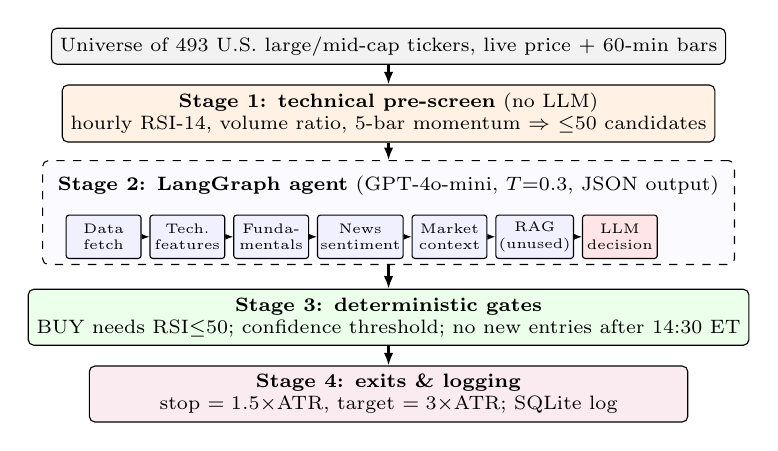
\begin{tikzpicture}[
  box/.style={draw, rounded corners=2pt, align=center, font=\scriptsize, minimum width=7.6cm, inner sep=3pt},
  node/.style={draw, fill=blue!6, rounded corners=1pt, font=\tiny, align=center, minimum width=0.95cm, minimum height=0.55cm, inner sep=1pt},
  arr/.style={-{Latex[length=1.6mm]}, thick}]
\node[box, fill=gray!10] (u) {Universe of \nScannerUniv{} U.S. large/mid-cap tickers, live price + 60-min bars};
\node[box, fill=orange!10, below=0.25cm of u] (s1) {\textbf{Stage 1: technical pre-screen} (no LLM)\\ hourly RSI-14, volume ratio, 5-bar momentum $\Rightarrow$ $\leq$50 candidates};
\node[font=\scriptsize, below=0.3cm of s1] (s2t) {\textbf{Stage 2: LangGraph agent} (GPT-4o-mini, $T{=}0.3$, JSON output)};
\node[node, below=0.12cm of s2t.south -| s1.west, anchor=north west, xshift=0.05cm] (n1) {Data\\fetch};
\node[node, right=0.1cm of n1] (n2) {Tech.\\features};
\node[node, right=0.1cm of n2] (n3) {Funda-\\mentals};
\node[node, right=0.1cm of n3] (n4) {News\\sentiment};
\node[node, right=0.1cm of n4] (n5) {Market\\context};
\node[node, right=0.1cm of n5] (n6) {RAG\\(unused)};
\node[node, right=0.1cm of n6, fill=red!10] (n7) {LLM\\decision};
\foreach \a/\b in {n1/n2,n2/n3,n3/n4,n4/n5,n5/n6,n6/n7} \draw[-{Latex[length=1mm]}] (\a) -- (\b);
\begin{scope}[on background layer]
\node[draw, dashed, fill=blue!2, rounded corners=2pt, fit=(s2t)(n1)(n7), inner sep=2pt] (s2) {};
\end{scope}
\node[box, fill=green!8, below=0.3cm of s2] (s3) {\textbf{Stage 3: deterministic gates}\\ BUY needs RSI$\le$50; confidence threshold; no new entries after 14:30 ET};
\node[box, fill=purple!8, below=0.25cm of s3] (s4) {\textbf{Stage 4: exits \& logging}\\ stop $=1.5\times$ATR, target $=3\times$ATR; SQLite log};
\draw[arr] (u) -- (s1); \draw[arr] (s1) -- (s2); \draw[arr] (s2) -- (s3); \draw[arr] (s3) -- (s4);
\end{tikzpicture}
\caption{Deployed four-stage pipeline. Only Stage~2 involves the LLM; FAP measures the incremental value of that stage's choice.}
\label{fig:arch}
\end{figure}

%──────────────────────────────────────────────────────────────────────────────
\section{The Forward Audit Protocol}
\label{sec:fap}
Every decision is logged at generation time, after the model's cutoff. We keep the first signal per (ticker, day, decision); multi-day entries are at the close of the signal day (robustness: next open), intraday entries at the close of the containing 60-minute bar. With $P_{s,t}$ the adjusted close and $\beta_{s,t}$ a 60-day rolling beta estimated before $t$, the beta-adjusted cumulative abnormal return is
\begin{equation}
\mathrm{CAR}_i(h)=\frac{P_{s_i,t_i+h}}{P_{s_i,t_i}}-1-\beta_{s_i,t_i}\Bigl(\frac{M_{t_i+h}}{M_{t_i}}-1\Bigr),
\end{equation}
$M$ being SPY~\cite{brown1985event}. Comparing against SPY or random stocks conflates the LLM's choice with the pre-screen's tilt toward oversold, volatile names, which carries its own reversal premium~\cite{jegadeesh1990evidence}. FAP instead builds, for each signal, a placebo of the $K{=}10$ stocks most similar on the same date but \emph{not} chosen, using $z$-scored nearest neighbours in feature space~\cite{daniel1997measuring} (daily RSI-14, 20-day momentum and ATR/price for multi-day signals; the pre-screen's own hourly features for intraday signals). The LLM's value-added is $\Delta_i(h)=\mathrm{CAR}_i(h)-\tfrac{1}{K}\sum_{j\in\mathcal{N}_K(i)}\mathrm{CAR}_j(h)$. Signals on the same day share market shocks and multi-day windows overlap, so FAP resamples non-overlapping $L{=}10$-day blocks (one day intraday) with replacement, $B{=}5{,}000$ times, reporting percentile 95\% CIs and two-sided bootstrap $p$-values; portfolio alphas use Newey--West errors~\cite{kunsch1989jackknife,newey1987simple}. A specification--deployment audit checks that the prompt's horizon, feature timeframe, exit levels and evaluated horizon agree~\cite{sculley2015hidden}, splitting return into selection (hold to horizon) and execution (deployed exit minus hold), replayed over a grid of stop/target multiples of daily ATR (stop assumed to fill first; gaps fill at the open; 10~bps round-trip costs throughout). A calibration audit treats stated confidence $c_i$ as $P(\text{beats SPY})$ and reports expected calibration error, Brier score against a constant forecast, and the block-bootstrapped Spearman correlation of $c_i$ with $\mathrm{CAR}_i(10)$~\cite{guo2017calibration}.

%──────────────────────────────────────────────────────────────────────────────
\section{Experimental Setup}
The log holds \nRaw{} decisions from \dFirst{} to \dLast{}. After de-duplication, \nBuy{} BUY signals on \nTick{} tickers over \nDays{} days have complete 10-day data, plus \iN{} intraday BUYs over \iDays{} days and \nWS{} WATCH~SELL signals as an overbought reference. Mean stated BUY confidence is \meanConf{}. The scanner's universe is \nScannerUniv{} U.S. large/mid-cap stocks (broader than the S\&P~500); \nNonIndex{} of \nLogTick{} logged tickers were non-members on 2026-01-01 (\nBuyNonIndexPct\% of evaluated BUYs). The placebo pool is the fixed \nIndexStart{}-member S\&P~500 as of 2026-01-01 (\nUniv{} with complete data); non-members are evaluated but never serve as placebo names, since an earlier, look-ahead version of the pool changed a regime-split result materially (repository). SPY returned \pct{\spyTotal} over the window. Because of the API outage (Section~\ref{sec:ops}), most signals come from April onward (\perFullN{} of \nBuy{}), so the usable window is about five months. Stage~3 changed stated confidence on \auStageChanged\% of BUYs and HOLDs were almost never stored (67 of \nRaw{}), so FAP measures the LLM \emph{plus its gates} against a placebo approximating, not replicating, its candidate set; \auTraced\% of database BUYs trace to a same-ticker log entry, a median \auOffset{} minutes earlier. With bootstrap SE of $\Delta$, the minimum detectable effect at 5\%/80\% power is $\mathrm{MDE}\approx2.80\,\mathrm{SE}$ (Table~\ref{tab:horizon}); a null means ``no edge larger than the MDE,'' not ``no edge.'' Section~\ref{sec:valid} measures size and power directly.

%──────────────────────────────────────────────────────────────────────────────
\section{Results}

\subsection{Selection: does the LLM pick better stocks?}
Table~\ref{tab:main} and Fig.~\ref{fig:event} give the central result. BUY signals earned \pct{\mBuyRawten} raw over ten days ($p{=}\mBuyRawtenP$), but market-adjusted CAR is indistinguishable from zero; the gap over the matched placebo is \pct{\mBuyMinusMatch} (CI \pct{\mBuyMinusMatchCI}). The placebo itself beats random by only $\mMatchMinusRand$\%, so the pre-screen's tilt carried no premium here either. Per-signal hit rates are not compared with the placebo's, since a $K$-stock average is positive more often than any single stock; the CAR gap above is the like-for-like measure.

\begin{figure}[t]
\centering
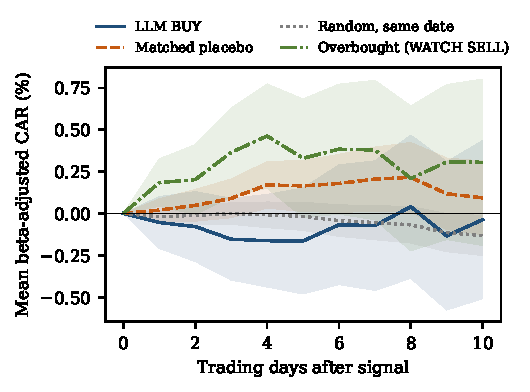
\includegraphics[width=\columnwidth]{figs/event_study.pdf}
\caption{Event study of beta-adjusted CAR after each signal. Bands are pointwise 95\% intervals that ignore dependence; Table~\ref{tab:main} reports block-bootstrap inference.}
\label{fig:event}
\end{figure}

\begin{table}[t]
\centering
\caption{Selection alpha of LLM BUY signals (10 trading days, \%)}
\label{tab:main}
\setlength{\tabcolsep}{2.5pt}
\begin{tabular}{@{}lrrcr@{}}
\toprule
Measure & $N$ & Mean & 95\% CI & $p$ \\
\midrule
LLM BUY, raw return & \nBuy & $\mBuyRawten$ & $\mBuyRawtenCI$ & \mBuyRawtenP \\
LLM BUY, excess over SPY & \nBuy & $\mBuyExten$ & $\mBuyExtenCI$ & \mBuyExtenP \\
LLM BUY, CAR & \nBuy & $\mBuyCarten$ & $\mBuyCartenCI$ & \mBuyCartenP \\
Matched placebo, CAR & \nBuy & $\mMatchCarten$ & $\mMatchCartenCI$ & \mMatchCartenP \\
Random same-date, CAR & \nBuy & $\mRandCarten$ & $\mRandCartenCI$ & \mRandCartenP \\
Overbought (WATCH SELL), CAR & \nWS & $\mWsCarten$ & $\mWsCartenCI$ & \mWsCartenP \\
\midrule
$\Delta$ LLM $-$ placebo & \nBuy & $\mBuyMinusMatch$ & $\mBuyMinusMatchCI$ & \mBuyMinusMatchP \\
$\Delta$ LLM $-$ random & \nBuy & $\mBuyMinusRand$ & $\mBuyMinusRandCI$ & \mBuyMinusRandP \\
\bottomrule
\end{tabular}
\end{table}

\textbf{Horizon robustness.} Table~\ref{tab:horizon} shows the null holds at every horizon, including the agent's native intraday one, and with next-open entry (excess over SPY: $\rNextOpenEx$\%, CI $\rNextOpenExCI$) or after dropping the most-oversold decile. Only the intraday test is sharp: its interval excludes any edge above \pct{\mdeUpperIntra}, below the 10~bps cost. At ten days the MDE is \pct{\mdeTen}, so an edge of 0.5\%/10 days ($\approx$13\%/yr if traded continuously) lies inside the interval: ``no edge larger than about \mdeTen\%,'' not ``no edge.'' In the intraday case, costs turn a zero-alpha strategy into a loss of \pct{\iHoldNet} per trade (CI \pct{\iHoldNetCI}).

\begin{table}[t]
\centering
\caption{LLM value-added $\Delta$ over the matched placebo by horizon, with the minimum detectable effect (MDE) at 5\%/80\% power (\%)}
\label{tab:horizon}
\begin{tabular}{@{}lrcr@{}}
\toprule
Horizon / variant & $\Delta$ & 95\% CI & MDE \\
\midrule
Intraday (bar close $\rightarrow$ 16:00 ET) & $\iAlpha$ & $\iAlphaCI$ & \mdeIntra \\
1 day & $\rHone$ & $\rHoneCI$ & \mdeOne \\
3 days & $\rHthree$ & $\rHthreeCI$ & \mdeThree \\
5 days & $\rHfive$ & $\rHfiveCI$ & \mdeFive \\
10 days & $\rHonezero$ & $\rHonezeroCI$ & \mdeTen \\
10 days, excl.\ most-oversold decile & $\rExclTopDecileRsi$ & $\rExclTopDecileRsiCI$ & -- \\
\bottomrule
\end{tabular}
\end{table}

\textbf{Do simple rules do as well?} On each of \baseDates{} BUY dates, four rules picked the same number of stocks from the fixed pool using one price-panel column and no model (Table~\ref{tab:baselines}). None is distinguishable from the LLM; the lowest-RSI rule is nominally best but its own interval spans zero.

\begin{table}[t]
\centering
\caption{10-day CAR (\%) of the \baseN{} LLM BUY signals and of rules picking the same number of stocks per date; last columns: LLM minus rule.}
\label{tab:baselines}
\footnotesize\setlength{\tabcolsep}{2pt}
\resizebox{\ifdim\width>\columnwidth\columnwidth\else\width\fi}{!}{%
\begin{tabular}{@{}lrcrc@{}}
\toprule
Strategy & Mean & 95\% CI & LLM $-$ rule & 95\% CI \\
\midrule
\baselinesRows
\bottomrule
\end{tabular}}
\end{table}

\subsection{Does the audit itself work?}\label{sec:valid}
We validated the inference on the real panel. \powSets{} fake, no-skill LLMs each picked, per BUY date, the same count at random from the 50 lowest-RSI names and were scored against the identical placebo (Table~\ref{tab:powersim}). Once centred, the procedures do not over-reject (block bootstrap: \powSizeBoot\% false-positive rate at nominal 5\%, cluster-robust $t$: \powSizeT\%, sign-flip: \powSizePerm\%; a 1~pp injected edge is found \powPwrOne\% of the time), but the ten-day placebo is biased for extreme picks: no-skill fakes earn \powBias{} pp over their placebo (SD \powSD{} pp), and the real LLM's \pct{\mBuyMinusMatch} lies below \powRealPct\% of them. Table~\ref{tab:sens} shows this is design-dependent, not a finding: under every placebo design the LLM's alpha stays within noise of zero (\sensLo{} to \sensHi{} pp, all spanning zero). The intraday result was validated the same way (\ipBlocks{} day-blocks): its false-positive rate is \ipSizeBoot\%, and unlike the ten-day case its placebo is essentially unbiased (\ipBias{} pp, SD \ipSD{} pp); across six designs the LLM's intraday alpha ranges $\ipLo$ to $\ipHi$ pp (all spanning zero), and it does worse than \ipWorseBase\% of no-skill pickers, suggestive rather than significant. The abstract's claim of no edge above $+0.035$\% intraday stands, with an empirical MDE of about \ipMDE{} pp.

\begin{table}[t]
\centering
\caption{Monte-Carlo check of the inference (\%): share of no-skill fake LLMs (\powSets{} ten-day, 300 intraday) reporting an edge, after centring, as a true edge $\delta$ is added ($\delta_0{=}0$: false-positive rate, nominal 5\%). $\delta$ (pp): ten-day 0/0.5/1.0/1.5/2.0; intraday 0/0.03/0.05/0.08/0.12.}
\label{tab:powersim}
\footnotesize\setlength{\tabcolsep}{2pt}
\resizebox{\ifdim\width>\columnwidth\columnwidth\else\width\fi}{!}{%
\begin{tabular}{@{}lccccc@{}}
\toprule
Procedure & $\delta_0$ & $\delta_1$ & $\delta_2$ & $\delta_3$ & $\delta_4$ \\
\midrule
\multicolumn{6}{@{}l}{\emph{Ten-day}} \\
\powRows
\midrule
\multicolumn{6}{@{}l}{\emph{Intraday}} \\
\ipPowRows
\bottomrule
\end{tabular}}
\end{table}

\begin{table}[t]
\centering
\caption{Sensitivity to the placebo's design (pp). LLM: alpha over the placebo, 95\% CI; No-skill: same quantity for random oversold pickers (the bias); last column: share (\%) of no-skill pickers the LLM does worse than.}
\label{tab:sens}
\footnotesize\setlength{\tabcolsep}{2pt}
\resizebox{\ifdim\width>\columnwidth\columnwidth\else\width\fi}{!}{%
\begin{tabular}{@{}lcccc@{}}
\toprule
Placebo design & LLM & No-skill & LLM $-$ bias & Worse than \\
\midrule
\multicolumn{5}{@{}l}{\emph{Ten-day (daily-feature placebo)}} \\
\sensRows
\midrule
\multicolumn{5}{@{}l}{\emph{Intraday (hourly-feature placebo)}} \\
\ipSensRows
\bottomrule
\end{tabular}}
\end{table}

\subsection{Consistency over time and a pre-registered forward test}
Splitting signal dates at 60\% (\fwdEarlyN{} signals / \fwdEarlyB{} blocks, then \fwdLateN{} / \fwdLateB{}) and evaluating six fixed hypotheses in each window (Table~\ref{tab:forward}) finds no detectable effect in either; the effective sample is \fwdAllB{} independent blocks, giving a smallest detectable difference of about \fwdMDE{} pp. H3 and H5 were suggested by development results, so these windows are exploratory for them. H6 is the primary skill test: ten-day alpha over the placebo minus its measured bias (Section~\ref{sec:valid}), fixed before any forward outcome existed. We pre-registered six hypotheses, thresholds and a minimum sample (\fwdNeedS{} matured signals, \fwdNeedB{} blocks) on 2026-09-25, and externally on the Open Science Framework the next day (osf.io/qhdgn, embargoed), adding a secondary hypothesis H7 on whether a stronger second model sorts the production BUYs. Below the minimum the test reports ``insufficient data.'' \fwdStatusText{} Four further exploratory analyses are in the project repository and none changes the conclusion: a purged walk-forward meta-model found no predictor of which BUYs beat their placebo (AUC at or below chance in both feature sets, including one with the LLM's own outputs added); an input ablation found only the technical-feature block moves decisions beyond the model's own run-to-run randomness; a signal-weighted portfolio simulation beat SPY on Sharpe ratio but not on alpha; and a post-hoc VIX/trend split found one nominally significant cell that reversed sign when an earlier, look-ahead placebo-pool bug was fixed, illustrating why it is reported as descriptive only.

\fwdStatusTable

\begin{table}[t]
\centering
\caption{Fixed hypotheses in the early/late development windows: 10-day CAR difference in \% (rank correlation for H2), 95\% CI.}
\label{tab:forward}
\footnotesize\setlength{\tabcolsep}{2pt}
\resizebox{\ifdim\width>\columnwidth\columnwidth\else\width\fi}{!}{%
\begin{tabular}{@{}lcc@{}}
\toprule
Hypothesis & Early window & Late window \\
\midrule
\forwardRows
\bottomrule
\end{tabular}}
\end{table}

\subsection{Specification--deployment mismatch and calibration}
The project targeted 5--10-day swing trades, but the consistency audit found production instead ran the \emph{intraday} prompt on 60-minute bars with 1.5$\times$ hourly-ATR stops, closing \prodEod\% of \prodN{} BUYs same-day. Replaying those levels on the intended ten-day hold (a counterfactual, since no position was ever held that long) shows \depStopRate\% would be stopped out, win rate falling from \holdWin\% to \depWin\% and mean net return from \pct{\holdNet} to \pct{\depNet}, a gap of \pct{\depGap} per trade (CI \pct{\depGapCI}, $p{=}\depGapP$); no stop/target in the replay grid beats simply holding. The realised, intraday-horizon counterpart is smaller: deployed levels stopped \iStop\% of trades and changed mean return by only \pct{\iDepGap} (CI \pct{\iDepGapCI}). On calibration: at the native intraday horizon, stated confidence averaged \iConf{} against \iHit{}\% of BUYs beating SPY (gap \iEce{}); at ten days, confidence concentrated at \calConf{} against only \calWin\% beating SPY, with ECE \ece{}, Brier \brier{} (worse than \brierBase{} constant) and rank correlation $\rho{=}\rhoConf$ (CI $\rhoConfCI$) with CAR; confidence does not even order trades, so gating on it (as Stage~3 does) is unfounded. Since Stage~3 alters \auStageChanged\% of BUY confidences, this audits the pipeline's confidence, not the model's alone; raw model confidence is logged separately from September 2026.

\subsection{Operational audit}
\label{sec:ops}
Of \opDecisions{} logged decisions across \opScans{} hourly scans, only \opReal{} (\opRealPct\%) came from the model; \opFallback{} were exception fallbacks, \opQuota{} of them caused by an exhausted OpenAI quota (``You exceeded your current quota'') on \opQuotaDays{} distinct days between \opQuotaFirst{} and \opQuotaLast{}, covering almost all of February and most of March; from April on, every decision reached the model. The API returned \opHttpLimited{} HTTP~429s against \opHttpOk{} successful completions; median latency to decision was \opLatMed{} s (95th pct.\ \opLatPtf{} s, five parallel workers). Signals before April ($n{=}$\perQuotaN{}) rest on very few independent blocks and show the only nominally significant $\Delta$ in the study; we do not interpret it, since it would not survive a Holm correction across the subset tests reported and comes from the least trustworthy sampling period. Stored rationales largely restate the pre-screen's oversold flag (\auCiteOversold\% of BUYs cite it, none contradicting the stored RSI), consistent with the null selection result; news and fundamentals scores stopped being logged after January, so their influence cannot be audited; fixing that logging gap is our first recommended change.

%──────────────────────────────────────────────────────────────────────────────
\section{Discussion}
\textbf{Lessons for AI engineering.} (1) \emph{Attribute before you celebrate}: the agent's portfolio simulation (repository) beat SPY on Sharpe, yet neither its alpha nor its spread over the placebo is distinguishable from zero: P\&L is a property of the whole pipeline. (2) \emph{Specification drift is a first-class failure mode}: one wrong flag sent an intraday prompt into production for a swing strategy, and every component behaved ``correctly'' in isolation while the counterfactual replay shows a \pct{\depGap}-per-trade loss on the intended horizon; consistency checks across prompt horizon, feature timeframe, exit rules and evaluation horizon belong in the test suite. (3) \emph{Do not gate on recorded confidence} unless calibrated on forward data, and log raw confidence separately from gated. (4) \emph{Log the failure path}: seven in ten decisions were silent fallbacks emitting a plausible-looking HOLD; fallbacks need their own label, counter and alert.

\textbf{Threats to validity.} The sample spans nine months, \nDays{} signal days and one 2024-vintage model, limiting power (Table~\ref{tab:horizon}) and generalisation to frontier models. The model was called by alias, and the served snapshot was unlogged until 2026-09-25, so a silent change cannot be excluded; decisions are stochastic (temperature 0.3; a pilot replay disagreed on 6.6\% of 38 candidates), so every result is one realisation. The matched placebo is biased for oversold picks (Section~\ref{sec:valid}). The placebo pool is reconstructed from two unaudited public sources and excludes \nNonIndex{} non-index tickers the scanner also traded; the scan universe changed after the study period (logged with the pre-registration). Stage-3 gates edit the LLM's output and HOLDs were not stored, so the audit measures the LLM plus its gates against an approximation of its candidate set. We assume 10~bps costs, no market impact and error-free bars; token counts were not logged. The external pre-registration (Data and Code Availability) is embargoed at the time of writing, so a reader can confirm only its filing date and identifier, not yet its content. FAP does not prove LLM agents cannot add value, only that this one did not do so measurably.

%──────────────────────────────────────────────────────────────────────────────
\section{Conclusion}
We ran a multi-agent LLM trading system in production after the model's knowledge cutoff and audited \nRaw{} logged decisions with the Forward Audit Protocol. Selection added no statistically detectable return over characteristic-matched alternatives at any horizon; a counterfactual replay shows deployed intraday stops would have turned the captured market drift into a flat result; recorded confidence was uninformative; and \opFallbackPct\% of decisions were quota-exhaustion fallbacks. FAP (contamination-free logging, matched placebos, block-bootstrap inference with stated power, consistency, calibration and operational audits) is cheap to adopt but validated on one system only, and its placebo needs a bias correction for extreme picks; we offer it as a starting point, not a settled standard. A purged walk-forward meta-model found no predictor of which calls work, and an input ablation showed only the technical block moves decisions beyond the model's own randomness. A pre-registered forward test (six hypotheses, plus a secondary H7 registered externally on OSF; minimum \fwdNeedS{} signals in \fwdNeedB{} blocks) is running and will be reported once it matures. Future work will compare frontier models under the same protocol.

\section*{Disclosures}
This system is a personal research project trading a paper (simulated) account only; no live capital was ever committed on its signals, and nothing here is investment advice. The work received no external funding, grant or sponsorship, and the author declares no financial conflicts of interest.

\section*{Data and Code Availability}
The code, tests, pre-registration and its addenda, the scripts generating every table and macro here, the analysis outputs and the decision log analysed (rationales included, news text excluded) are in a public release of the project (repository URL and archive DOI to be added at submission). Raw Yahoo Finance price data are not redistributed under the provider's terms; the scripts re-download them (headline statistics agree to about eight decimals across downloads). The forward test was also registered externally on OSF on 26 September 2026, before any forward outcome had matured (osf.io/qhdgn, embargoed until submission), independent of the author's own repository timestamps.

%──────────────────────────────────────────────────────────────────────────────

\bibliographystyle{IEEEtran}
\bibliography{refs}

\end{document}
